\documentclass{article}
%\documentclass{article}

\usepackage{tikz}
\usetikzlibrary{external}

\usepackage{braket}

\usepackage{subcaption} % Subfigure environment 
\usepackage{gensymb}

\usepackage{amsmath} % Mathematical symbols
\usepackage{amssymb} % Symbols

\usepackage{caption}% Captions onder figuur gecentreerd
%\usepackage[toc,page]{appendix}
\usepackage{subcaption} % Subfigure environment 
%\usepackage{float}

\usepackage{etoolbox} %for if empty functionality

\usepackage{ifthen}

%break long urls at a - and not only at . or /
\usepackage{url}
\def\UrlBreaks{\do\/\do-}
\usepackage{breakurl}
\usepackage[hidelinks,breaklinks]{hyperref}

\usepackage{verbatim}
%\usepackage{hyperref}
\usepackage{siunitx} % Elegant eenheden zetten
\usepackage[version=3]{mhchem} % ingeven van chemische fomules
\usepackage{cleveref} % Paragraaf tekens
\usepackage{longtable}
%\usepackage{lscape}
\usepackage[T1]{fontenc}
\usepackage{fontenc}
\usepackage{amsfonts}
\usepackage{mathtools}
\usepackage{grffile}%double dot in figure name
\usepackage{lipsum}
\usepackage{siunitx}
\usepackage{xcolor}
\usepackage{sectsty}
\usepackage{booktabs}
\usepackage{physics}
\usepackage{leftidx}
\usepackage[utf8]{inputenc}
\usepackage{gensymb} % /textdegree


%\setcounter{tocdepth}{4}
\setcounter{secnumdepth}{4}

\usepackage{graphicx}

\usepackage{todonotes}

%\usepackage[nottoc]{tocbibind}

\title{Thesis}

\date{2020}

\begin{document}

%\def\temp{#1}\ifx\temp\empty
%  <EMPTY>%
%\else
%  <NON EMPTY>%
%\fi




%use first argument is numbers of O's, second the labels, can be empty
%\mpo{3}{ {0,1,2,3,4} }

\newcommand{\combineTikz}[3]{
	\begin{tikzpicture}[baseline={0-0.5*height("$=$")}]
		\node (AA) at (0,0)  { #1   };
		\node (AB) at ( {#3} ,0)  {  #2  };
	\end{tikzpicture}
}


\newcommand{\mpo}[6]  { \begin{tikzpicture}[baseline={0-0.5*height("$=$")}]
        	%\def \NNodes {#1}
			%\def \NodeName {#2}          
			%\def \NameUp   {#3} 
			%\def \NameDown  {#4}	

			\def \legLength {0.6}
        	\def \radius {0.3}

        	\pgfmathsetmacro{\step}{2*\radius+\legLength}
        	\pgfmathsetmacro{\legpos}{\radius+\legLength}
        
        	\pgfmathsetmacro{\Nmax}{#1-1}
        
        	\foreach \N in {0,..., \Nmax }{
        		\pgfmathsetmacro{\p}{\N*\step}

                % up and down labels
                \def\temp{#3}\ifx\temp\empty
                  \def \labelUp {}
                \else
                 \pgfmathsetmacro{\labelUp}{  {#3}[\N]  }
                \fi

                \def\tempp{#4}\ifx\tempp\empty
                  \def \labeldown {}
                \else
                 \pgfmathsetmacro{\labeldown}{  {#4}[\N]  }
                \fi


				\def\aab{#5}\ifx\aab\empty
	                  \def \dotssite {0}
                \else
	                 \pgfmathsetmacro{\dotssite}{  {#5}[\N]  }
                \fi

				\ifthenelse{\dotssite = 0}{
				    
				    \def\aac{#6}\ifx\aac\empty
    	                  \def \nname {O}
                    \else
    	                 \pgfmathsetmacro{\nname}{  {#6}[\N]  }
                    \fi
				    
				    
				
					\node[circle,draw, radius=\radius] (O\N) at (\p,0) {\nname};
        		
        		
	                \node[] (Ou\N) at (\p, \legpos ) { \labelUp };
	
	
	                \node[] (Od\N) at (\p,-\legpos) {\labeldown};
	           
	        
	        		\draw (O\N) -- (Ou\N);
	        		\draw (O\N) -- (Od\N);
				}{
					\node[circle] (O\N) at (\p,0) { $\cdots$ };
        		
        	
				}
        
        		
        	}
        
            \ifthenelse{  #1  =1  }{}{
                \foreach \N in {1,...,\Nmax }{
            		\pgfmathsetmacro{\M}{\N-1}
    				\pgfmathsetmacro{\label}{ {#2}[\N]  }
					%\pgfmathsetmacro{\label}{ 5}

            		\draw (O\M) --  node[above]  {\label} (O\N);
            	}
            }
        
			\pgfmathsetmacro{\labelo}{ {#2}[0]}
			\pgfmathsetmacro{\labeli}{  {#2}[\Nmax+1]}

        	\node (N0) at (-\legpos,0) {};
        	\draw (N0) -- node[above] {\labelo} (O0);
        	
        	\pgfmathsetmacro{\endpos}{\step*\Nmax+\legpos}
        
        	\node (Ne) at (\endpos,0) {};
        	\draw (Ne) -- node[above] {\labeli} (O\Nmax);
        
        	%\draw (O0) --  node[above] {1} (O1);
        

\end{tikzpicture}}

\newcommand{\expH}[5]{ \begin{tikzpicture}[baseline={0-0.5*height("$=$")}]
            
			\def \NNodes {#1};
		
			
			\def\aaa{#2}\ifx\aaa\empty
              \def \text { $e^{-\beta \hat{H}_{\NNodes} }$ }
            \else
              \def \text {#2}
            \fi
			
			\pgfmathwidth{ "\text" }
            \def \textwidth { \pgfmathresult }

			
			%\pgfmathsetmacro{\text}{width(\text)}
			
        	\def \legLength {0.6}
        	\def \radius {0.3} %fix to fit text inside for size 1
			\def \boxHeight {0.4};

        	\pgfmathsetmacro{\step}{2*\radius+\legLength}
        	\pgfmathsetmacro{\legpos}{\radius+\legLength}
        	\pgfmathsetmacro{\dotpos}{\boxHeight+\legLength/2}
        
        	\pgfmathsetmacro{\Nmax}{\NNodes -1}
        
            
        
			\pgfmathsetmacro{\boxsize}{ max ( \textwidth/1cm , \step*\Nmax )   + \radius}
			
			%\pgfmathsetmacro{\boxsize}{ 5  )}
			%\pgfmathsetlength{\boxsize}{ max( \textwidth,  \boxsize1  )}

			

%            \ifthenelse{#1=1}{
%                \def \left {-0.6}
%                \def \right {0.6}
%            }{
                \def \left {-\radius}
                \def \right {\boxsize}
%            }

			\draw (\left,- \boxHeight ) rectangle (\right, \boxHeight ) [add reference =H] ; 
			
			
        	\node  at (H center) { \text };
        
        	\foreach \N in {0,..., \Nmax }{
        		\pgfmathsetmacro{\p}{\N*\step}
        		
        		% up and down labels
                \def\temp{#3}\ifx\temp\empty
                  \def \labelUp {}
                \else
                 \pgfmathsetmacro{\labelUp}{  {#3}[\N]  }
                \fi

                \def\tempp{#4}\ifx\tempp\empty
                  \def \labeldown {}
                \else
                 \pgfmathsetmacro{\labeldown}{  {#4}[\N]  }
                \fi
        		
        
        		\node[] (O\N) at (\p,0) {};
        		
        		
        		\ifthenelse{ \equal{\labelUp}{...}  }{
        		    \node[] (Ou\N) at (\p, \dotpos ) {\labelUp};
        		}{
        		  \node[] (Ou\N) at (\p, \legpos ) {\labelUp};
        		   \draw (Ou\N) --  (Ou\N  |- H north);
        		}
        		
        		
        		\ifthenelse{ \equal{\labeldown}{...}  }{
        		    \node[] (Od\N) at (\p,-\dotpos ) {\labeldown};
        		}{
        		  \node[] (Od\N) at (\p,-\legpos) {\labeldown};
                   \draw (Od\N) --  (Od\N  |- H south);
        		}
        		
        		


        		
        		
        	}
        	
        	\def\tempt{#5}\ifx\tempt\empty
                  
            \else
             	\pgfmathsetmacro{\labelo}{ {#5}[0] }
    			\pgfmathsetmacro{\labeli}{  {#5}[1] }
    			
    			\pgfmathsetmacro{\leftleg}{  \left - \legLength }
    			\pgfmathsetmacro{\rightleg}{  \right + \legLength }
    
            	\node (N0) at (\leftleg,0) {\labelo};
            	\draw (N0) -- ( N0  -| H west);
            	
            	\node (Ne) at (\rightleg,0) {\labeli};
            	\draw (Ne) --  ( Ne  -| H east);
            \fi
        	

   \end{tikzpicture} }




\onecolumn
\begin{titlepage}
	\begin{center}	
		
		\pagenumbering{gobble}
		
\includegraphics[width=4cm]{Figuren/UGent.png} \\[0.5cm]    %Logo UGENT	
		
		\Large{\textsc{Master Engineering Physics}} \\[0.5cm]  %Vakgroep	
		
		\normalsize{Year 2020-2021} \\[3cm]  %Academiejaar
		
		\huge{\textsc{Master desertatoin}} \\[0.25cm]   %Titel
		
		\Large{\textsc{Thesis Tensor networks}}\\[0.25cm]
		
		\large \textnormal{October 2020} \\[2.5cm]   %Extra informatie
		
		%\small      %Namen
		
       David Devoogdt \\       [2.5cm]

		 
        Academic supervisor: prof. 
         

		
		
		\vfill		
		
	\end{center}
\end{titlepage}

\tableofcontents

\newpage
\listoftodos
\newpage

%\twocolumn
\pagenumbering{arabic}

\tikzset{add reference/.style={insert path={%
                    coordinate [pos=0,xshift=-0.5\pgflinewidth,yshift=-0.5\pgflinewidth] (#1 south west)
                    coordinate [pos=1,xshift=0.5\pgflinewidth,yshift=0.5\pgflinewidth]   (#1 north east)
                    coordinate [pos=.5] (#1 center)
                    (#1 south west |- #1 north east)     coordinate (#1 north west)
                    (#1 center     |- #1 north east)     coordinate (#1 north)
                    (#1 center     |- #1 south west)     coordinate (#1 south)
                    (#1 south west -| #1 north east)     coordinate (#1 south east)
                    (#1 center     -| #1 south west)     coordinate (#1 west)
                    (#1 center     -| #1 north east)     coordinate (#1 east)
                }}}

\section{Introduction}
\todo{write this}

To deal with these strongly correlated systems, a class of methods called tensor networs were introced.

The Hilbert space grows exponentially with system size.

Want to be able to model various Hamiltonians (e.g. Bosons and
Fermions).
Want to avoid the sign problem of quantum Monte Carlo.
Want to measure physical properties and observables

\subsection{Quantum monte carlo}

\section{Statistical mechanics}

\subsection{Statistical mechanics}

The physics of a system in thermodynamical equilibrium can be derived from it's partition function Z.
\begin{equation}
    \begin{split}
        Z &= \sum e^{ - \beta E_n} \\
        &= \sum_n \Braket{n | e^{ - \beta \hat{H} }  | n} \\
        &= \Tr( e^{ - \beta \hat{H} } )
    \end{split}
\end{equation}
The first line is the partition function for clasical discrete systems. The index n runs of all possible microstates. It is know that the propability to find the system in a given microstates is given by:
\begin{equation}
    p_i = \frac{\sum e^{ - \beta E_i}}{Z}
\end{equation}
An useful quantity is the density matrix $\rho$.
\begin{equation}
    \begin{split}
        \rho &= \sum_j p_i  \Ket{ \Psi_j} \Bra{\Psi_j}   \\
        &= \sum_j \frac{ e^{ - \beta \hat{H} } }{Z}  \Ket{ \Psi_j} \Bra{\Psi_j}
    \end{split}
\end{equation}
With this notation
\begin{equation}
    \begin{split}
        Z &= \Tr( \rho) \\
        \Braket{X} &= \Tr(\rho \hat{X})
    \end{split}
\end{equation}

\subsection{Time evolutions}

\subsection{Tensor network methods}

% https://arxiv.org/pdf/1901.05824.pdf

\subsubsection{Approximations to  \texorpdfstring{$ \hat{U}(\delta)$}{U}   }

TEBD, MPO $W^{I,II}$

\subsubsection{global Krylov method }

\subsubsection{MPS-local methods }
local Krylov
TDVP

\section{contruction MPO}

\subsection{Type A}
This type was originally proposed in \cite{Vanhecke2021}. The first few blocks in the expansion are the following:

\begin{equation}
    \begin{split}
        &\mpob{1}{ {,}  }{}{}{}{{,,}} \\
        &\mpob{2}{ {,"1",}  }{}{}{}{{,,}}\\
        &\mpob{3}{ {,"1","1",}  }{}{}{}{{,,,}}\\
        &\mpob{4}{ {,"1","2","1",}  }{}{}{}{{,,,,,}}\\
        &\mpob{5}{ {,"1","2","2","1",}  }{}{}{}{{,,,,,}}\\
    \end{split}
\end{equation}

The following types of blocks appear in the cluster expansion

\mpo{1}{ {"n","m"}  }{}{}{}{},\mpo{1}{ {"m ","n"}  }{}{}{}{} and \mpo{1}{ {"n","n"}  }{}{}{}{} with $n \in \mathbb{N}_0$ and $m=n-1$.

The $O^{n n}$ block is in defined for a chain with an odd number of sites. The contraction of $O^{n m }$ and $O^{m n} $ is defined by for a chain with even order. The decomposition is defined up to a gauge transformation.

\paragraph{Dimension}

In this scheme, virtual level n has dimension $d^n$. Of course, this dimension can be lowered if some error is allowed for the longest chain.

\paragraph{discussion}

Type A can form long chains, which where not explicitly optimised for. The question arise whether this will results in accurate results for cyclic systems or not.

\subsection{Type B}

Type B only contains blocks of the following form; $O^{m n}$ and $O^{n 0}$.The first few blocks are:
\begin{equation}
    \begin{split}
        &\mpob{1}{ {,}  }{}{}{}{{,,}} \\
        &\mpob{2}{ {,"1",}  }{}{}{}{{,,}}\\
        &\mpob{3}{ {,"1","1",}  }{}{}{}{{,,,}}\\
        &\mpob{4}{ {,"1","2","3",}  }{}{}{}{{,,,,,}}\\
        &\mpob{5}{ {,"1","2","3","4",}  }{}{}{}{{,,,,,}}\\
    \end{split}
\end{equation}

\def \rhs{\expH{2}{ $L_{m}^{-1}  M_{n+1} $ }{{"$i_n$","$i_{n+1}$"}}{{"$j_n$","$j_{n+1}$"}}{{"m","0"}}  }
\begin{equation}
    \begin{split}
        \mpo{2}{ {"m","n","0"}  }{ { "$i_n$","$i_{n+1}$"}}{ { "$j_n$","$j_{n+1}$"}}{}{} =  U^n  \Sigma V^{\dagger}\\
    \end{split}
\end{equation}

The following split is made: $O^{m n} \cong U^n$ and $O^{n 0} \cong  \Sigma V^{\dagger}$. In this way the left inverse exists and doesn't need any calculation: $O^{m n} = U^{\dagger}$.

\paragraph{dimension} From the construction the bond dimension grows from the left to the right. For the last step, there are only $d^2$ non zero singular values.  Each steps adds $d^2$ to the dimension.
For the last step, only $d^2$ non zero singular values need to be keeped. With the following natation:
\begin{equation}
    \begin{split}
        \mpo{1}{ {"m","n"}  }{ { "\(i\)",}}{ { "$j$",}}{}{} &= A^m_{ (\alpha i j ) \beta} \\
        \mpo{1}{ {"n","0"}  }{ { "$i$",}}{ { "$j$",}}{}{} &= B^n_{ (\alpha i j ) \beta} \\
    \end{split}
\end{equation}
The bond dimension of lower virtual levels can be reduced if we can solve the following equations simultaneously:

Then the MPO doesn't change if there are matrices $A'^{n}$, $A'^{n+1}$ and $B'^{n}$ such that
\begin{equation}
    \begin{split}
        S=A^{m} A^{n} &= A'^{m} A'^{n} \\
        T=A^{m} B^{n} &= A'^{m} B'^{n} \\
    \end{split}
\end{equation}
Such matrices with optimal bond dimension can be found with generalised SVD. Generalised SVD decomposes 2 matrices as follows:
\begin{equation}
    \begin{split}
        S^{\dagger} = (U \Sigma_1) Q^{\dagger} \\
        T^{\dagger} = (V \Sigma_2) Q^{\dagger}
    \end{split}
\end{equation}
The new bond dimension is the $\dim{n'} =d^2 \cdot \min( \dim{n-1}, \dim (n+1) )$.  This is higher than the dimension of type A.

\paragraph{Discussion}
The bond dimension is larger than type A, but the long chains from A are absent. The left inverse is always well defined and doesn't need any computation, because hermitian matrix U can be inverted easily. One major drawback is that for long chains, the virtula bonds are very large before they can be shrunk with the gsvd procedure.

\subsection{Type C}
\todo{primed virtual levels}

This type implements the same strict type as Type B, but in a different way. No calculation is involved, except the calculation of the the exponentiated hamiltonian to certain order. The following kind of MPO strings are allowed:

\begin{equation}
    \begin{split}
        &\mpob{1}{ {,}  }{}{}{}{{,,}} \\
        &\mpob{2}{ {,"1",}  }{}{}{}{{,,}}\\
        &\mpob{3}{ {,"1'","1'",}  }{}{}{}{{,,,}}\\
        &\mpob{4}{ {,"1''","2''","3''",}  }{}{}{}{{,,,,,}}\\
        &\mpob{5}{ {,"1'''","2'''","3'''","4'''",}  }{}{}{}{{,,,,,}}\\
    \end{split}
\end{equation}
and so forth. All but one MPO elements are chosen to be the identity matrix. The middle one is the exponentiated hamiltonian with reshaped legs.

\paragraph{discussion}
As can be expected from the construction, the bond dimension grows very fast. This type is just as precise as Type B.

\subsection{Type D}

This type uses a differemt setup which tries to capture the best of both Type A and B. Type  could handle long range correlation better because of the introuction of $O^{n n}$, but the inverse was not necesarily well defined. Type B had well conditioned inverses, but performed in most of the cases worse. The block appearing in type D are as follows:

\mpo{3}{{"m","n","n","m"}}{{,"-",}}{{,"-",}}{}{{"O","$D_n$","O"}} and \mpo{1}{{"n","n"}}{}{}{}{}

Similar to type A,

\def \rhs{\expH{2}{ $L_{n}^{-1}  M_{2n+2}  R_{n}^{-1}$ }{}{}{{"n","n"}}  }
\begin{equation}
    \begin{split}
        \mpo{3}{{"m","n","n","m"}}{{,"-",}}{{,"-",}}{}{{"O","$D_n$","O"}} &= \rhs \\
        &= U \Sigma V^{ \dagger}
    \end{split}
    \label{eq_nmn_level}
\end{equation}

Matrix $D_n$ is the singular value diagonal matrix devided by a normalisation factor $\phi$. Both U and V are multiplied by $  \sqrt{\phi} $.

\paragraph{discussion}
It's not completely clear what the values of $\phi$ should be.  If $\phi$ is to large, large chains are not surpressed. If phi is to small, the $O^{n n}$ blocks will become large and hence the chain will diverge again. A reasonable value is the sum of the singular values. \todo{other things could be tried here, WIP}

\paragraph{matrisation}
The cost of this type lies in the fact that it has no compact way of casting it to a matrix. The following works, but has quite a large dimension:

\begin{tabular}{ccc|cc|cc|cc}
    $O_{00}$               & $O_{01} $   &             & $-2  O_{01}$ &                & $ O_{01}$ &             & $ O_{01}  D_1^{1/2}$           &                                \\
    ${O_{10}}$             &             & ${ O_{12}}$ &              & $-2 { O_{12}}$ &           & ${ O_{12}}$ &                                &                                \\
                           & ${ O_{21}}$ &             &              &                &           &             &                                &                                \\
    \hline
    ${O_{10}}$             &             &             &              &                &           &             &                                &                                \\
                           & ${ O_{21}}$ &             &              &                &           &             &                                &                                \\
    \hline
    ${ O_{10}}$            &             &             &              &                & $O_{11}$  &             &                                &                                \\
                           & ${ O_{21}}$ &             &              &                &           & $O_{22}$    &                                &                                \\
    \hline
    $ D_1^{1/2} { O_{10}}$ &             &             &              &                &           &             &                                & $D_1^{-1/2} O_{12}  D_2^{1/2}$ \\
                           &             &             &              &                &           &             & $ D_2^{1/2} O_{21} D_1^{-1/2}$                                  \\\end{tabular}

\todo{fix this }

\subsection{Type E}

Again, this is a strict variant which needs exactly twice the bond dimension of type A. The idea is to split every chain in a left and a right part. For the left part, the numbers increase while right part they decrease. This construction carries over well to higher dimensions. The first few blocks are:
\begin{equation}
    \begin{split}
        &\mpob{1}{ {,}  }{}{}{}{{,,}} \\
        &\mpob{2}{ {,"1",}  }{}{}{}{{,,}}\\
        &\mpob{3}{ {,"1","1'",}  }{}{}{}{{,,,}}\\
        &\mpob{4}{ {,"1","2","1'",}  }{}{}{}{{,,,,,}}\\
        &\mpob{5}{ {,"1","2","2'","1'",}  }{}{}{}{{,,,,,}}\\
    \end{split}
\end{equation}
The construction is very similar to type A


\section{Benchmark 1D cluster expansion}
The goal of numerical techniques is to simulate the physics of real world systems. These are, to some extend, captured by different models. Models are a simplified mathematical description that captures some relevant physics of more complicated systems. This section introduces some specific models, their relevance and some properties. These models will be used later te benchmark the developed tensor network expansion.

\subsection{Ising model}

The prototypical example of a model in the field of strongly correlated matter is the Ising model. It was first introduced 1925 by Ernest Ising, as a model to capture ferromagnetism. He proved that for a linear chain, there is no phase transition at finite temperature. He wrongly concluded that this would also be the case in higher dimensions, but it turned out t be one of the deepest and far-reaching problems in 20th century \cite{Taroni2015}.

The Ising model, in essence, assigns an energy contribution to neighbouring spins. These spins sit on a fixed position on a chain (1D) or lattice (2D/3D/...). In classical Ising, the operators in the Hamiltonian all commute with each other. An energy is assign between neighbouring spins and possible and energy for alignment with an external magnitic field in the same direction. In quantum Ising model, a transversal field is added. Often, the particles on the grid are spin 1/2 particles, but of course other particles are possible.

Many generalizations exist for the Ising model. \todo{q potts,...}

\subsubsection{Classical Ising}

The classical ising model is given by the following hamiltonian:
\begin{equation}
    H = -J \left (  \sum_{<i j>} \sigma_i \sigma_j + h \sum_i \sigma_i \right )
\end{equation}
where $<i j>$ runs over all neighbouring lattice sites. The possible values of $\sigma$ depends on the spin dimension. For spin $1/2$ lattices $\sigma \in {-1,+1}$. g encodes the interaction strength of the external magnetic field.

The sign J determines the low temperature ground state. A positive J will tend to allign all neighbouring spins at low temperature. This is often called ferromagnetic, because all the aligned spins cause a macroscopic magnitisation. On the other hand, a negative J causes neighbouring spins to have an opposite sign.

Depending on the sign of the longitudinal field h, the spins tend to align or anti align with this external field. This lifts the degeneracy of the groundstate.

\paragraph{1D}

The classical 1D model was solved analytically by Lens. \todo{blabla}

\paragraph{2D}

In 2D, it becomes important to define the lattice. Here, and in the simulations, we will consider a square lattice. This model was famously solved by Lars Onsager in 1944, by using the transfer matrix method. In 2 dimensions, the Ising model has a phase transition at finite temperature. The critical temperature is $T_c = \frac{2 J}{T ln( \sqrt{2}+1)}$.

Only the $h=0$ case the is solved analytically. For higher dimensions, no analytical solution is known. For these cases, we need to use numerical techniques if we want to understand the behaviour of these models.

On different lattices, interesting thins can happen. For instance, the groundstate of an antiferromagnet on a triangular lattice is not obvious to determine. The spins tend to antiallign, but at least 2 of 3 spins on the corner of a triangle have to align. Remarkably, as will be explained in \cref{sec:PhasesAndCrit}, the physics at the phase transition does remain invariant when the lattice is changed.

\subsubsection{Quantum Ising}

As we all know, the real world behaves, certainly at small length and time scales, quantum mechanically. Therefore, it is important to understand how the quantum Ising model differs from the classical model. In the quantum Ising model, the operators no longer commute with each other. An example is the transversal Ising model given by the following hamiltonian:

\begin{equation}
    \hat{H} = -J \left (  \sum_{<i j>} \sigma^x_i \sigma^x_j + g \sum_i \sigma^z_i \right )
\end{equation}

In the case that $g=0$, this is the classical Ising model (in the $h=0$ case).

\paragraph{1D}
Different to the classical case, the 1D model already contains a phase transition.

\paragraph{2D}

\begin{figure}
    \center
    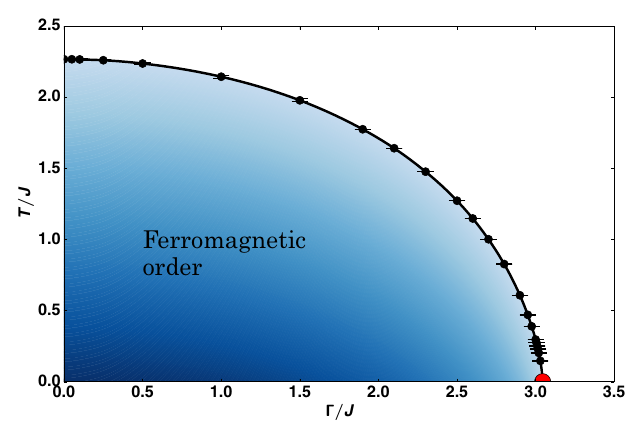
\includegraphics[width=\textwidth]{Figuren/phsyics/2disingphase.png}
    \caption{Phase diagram for 2D transversal Ising model. Figure taken from \cite{Hesselmann2016}}
    \label{2dtisingphasediag}
\end{figure}

\subsection{Heisenberg}

The heisenberg model is given by:

\begin{equation}
    \hat{H} =  -\left( \sum_{<i j>} J_x \sigma^z_i \sigma^z_j + J_y \sigma^y_i \sigma^y_j+ J_z \sigma^z_i \sigma^z_j + h \sum_i \sigma^z_i \right )
\end{equation}

These models have different names depending on the values of $J_{\alpha} $ with $\alpha=x,y,z$. $J_x = J_y \neq J_z = \Delta$ is called the XXZ model.

\subsection{Random}
It's also possible to construct random hamiltonians. \todo{in basis: hermitian H}

\bibliographystyle{elsarticle-num} 
\bibliography{bib}
\end{document}
